%TEX root = ../dissertation.tex

\chapter{Implementation}
\label{chapter:implementation}
In chapter \ref{chapter:solution}, we have presented the solution, that is,
the mobile apps that owners and end users need and the \gls{API} that developers use
to develop proximity-based mobile apps for this two kinds of users.
This chapter explaines the implementation of each part of the solution
(tools, programming languages, etc). Since there are two examples that were
created to test the concept, we will dive into their implementation also.
The code is hosted on
github\footnote{http://github.com/}, which is a hosting service for projects
that use git\footnote{http://git-scm.com/}, as their \gls{VCS}.

Next, in section \ref{sec:implementation_tools}, there is a summary of tools that were used in the development of the Smart Places solution.
Then, section \ref{sec:implementation_tags}, explains the technology that was used to support the existence of tags, according to our definition of a Smart Place.
Section \ref{sec:implementation_backend} presents the backend and the domain model that it is stored and managed.
Each Smart Place has its own code and offers a proximity-based service, such as the ones provided by the Smart Restaurant and Smart Museum examples, introduced in chapter \ref{chapter:solution}, section \ref{sec:solution_examples}.
The way our solution allows the user to have access to Smart Places is described in section \ref{sec:implementation_smart_places}.
The implementation of the mobile apps, for owners and end users, is presented in section \ref{sec:implementation_mobile_applications}.
In section \ref{sec:implementation_developers_api} we describe the implementation of the \gls{API} for developers.
In section \ref{sec:implementation_examples} we explain how the Smart Restaurant and Smart Museum examples were developed.
Last, section \ref{sec:implementation_summary} concludes this chapter.

\section{Tools}
\label{sec:implementation_tools}
During the development of our solution, several tools were used.
The components, such as, the backend, mobile apps, the Developers \gls{API} and the examples, were developed using different tools, from development environments to build and dependency management tools.

Since this solution needs to store information about each beacon, we
needed a backend to be able to change this information without having
to change the mobile apps.
However, this backend just has to be able to store data and retrieve that
data when client applications request it.
Instead of implementing this component from the scratch, we used
Parse\footnote{https://parse.com}, which is a \glsfirst{BaaS}.
It provides a dashboard, where developers can create classes
and define their fields and the type of each field, which can be a string,
a number, a boolean, a pointer to another object, a \gls{JSON} object, etc.

For the Android apps, we have used the following tools:
\begin{description}
  \item[Android Studio] \footnote{http://developer.android.com/sdk/index.html} is an \gls{IDE}, based on IntelliJ\footnote{http://www.jetbrains.com/idea},
  to develop Android
  applications;
  \item[Java] was the programming language that was used to write the code of the mobile apps.
\end{description}

The Javascript \gls{API} and the Smart Restaurant and Smart Museum examples were created using web technologies, such as \gls{HTML}, \gls{CSS} and Javascript.
However, besides these languages, we have used tools to manage the build process and also the necessary dependencies:
\begin{description}
  \item[Bower]\footnote{http://bower.io} is a tool used in web applications, to manage frontend dependencies. It was used here to manage dependencies of our Smart Restaurant and Smart Museum examples.
  Also, it was used in our Javascript \gls{API} to allow this \gls{API} to be released as a library in order to make it avaible, to install, using this tool;
  \item[Grunt]\footnote{http://gruntjs.com} is another tool used in web applications, to manage the build process of frontend assets.
  It is based on tasks that are added depending on the needs of the project.
  There are tasks available to concatenate all Javascript files in just one, minify Javascript files, copy files, etc.
\end{description}

\section{Tags}
\label{sec:implementation_tags}
According to our definition of Smart Place, we need to tag objects to provide proximity-based services.
Several location technologies were presented in chapter \ref{chapter:background}.
To support the existence of tags, we chose \gls{BLE} Beacons using the ibeacon protocol, because most smartphones are \gls{BLE} enabled and it does not require the user to acquire any extra hardware.
We have used three beacons from Estimote\footnote{http://estimote.com}
(Figure \ref{fig:estimote}), that come with a development kit.
In this kit, each beacon come with a name, defined by \tm{Estimote}.
The blue, green and purple are named ice, mint and blueberry, respectively.
Besides the hardware, this product offers a \gls{SDK} for Android and
iOS. It also has a cloud service where developers can set and get
some information about each beacon, such as, the \gls{UUID}, name, etc.

\begin{figure}[!ht]
  \centering
    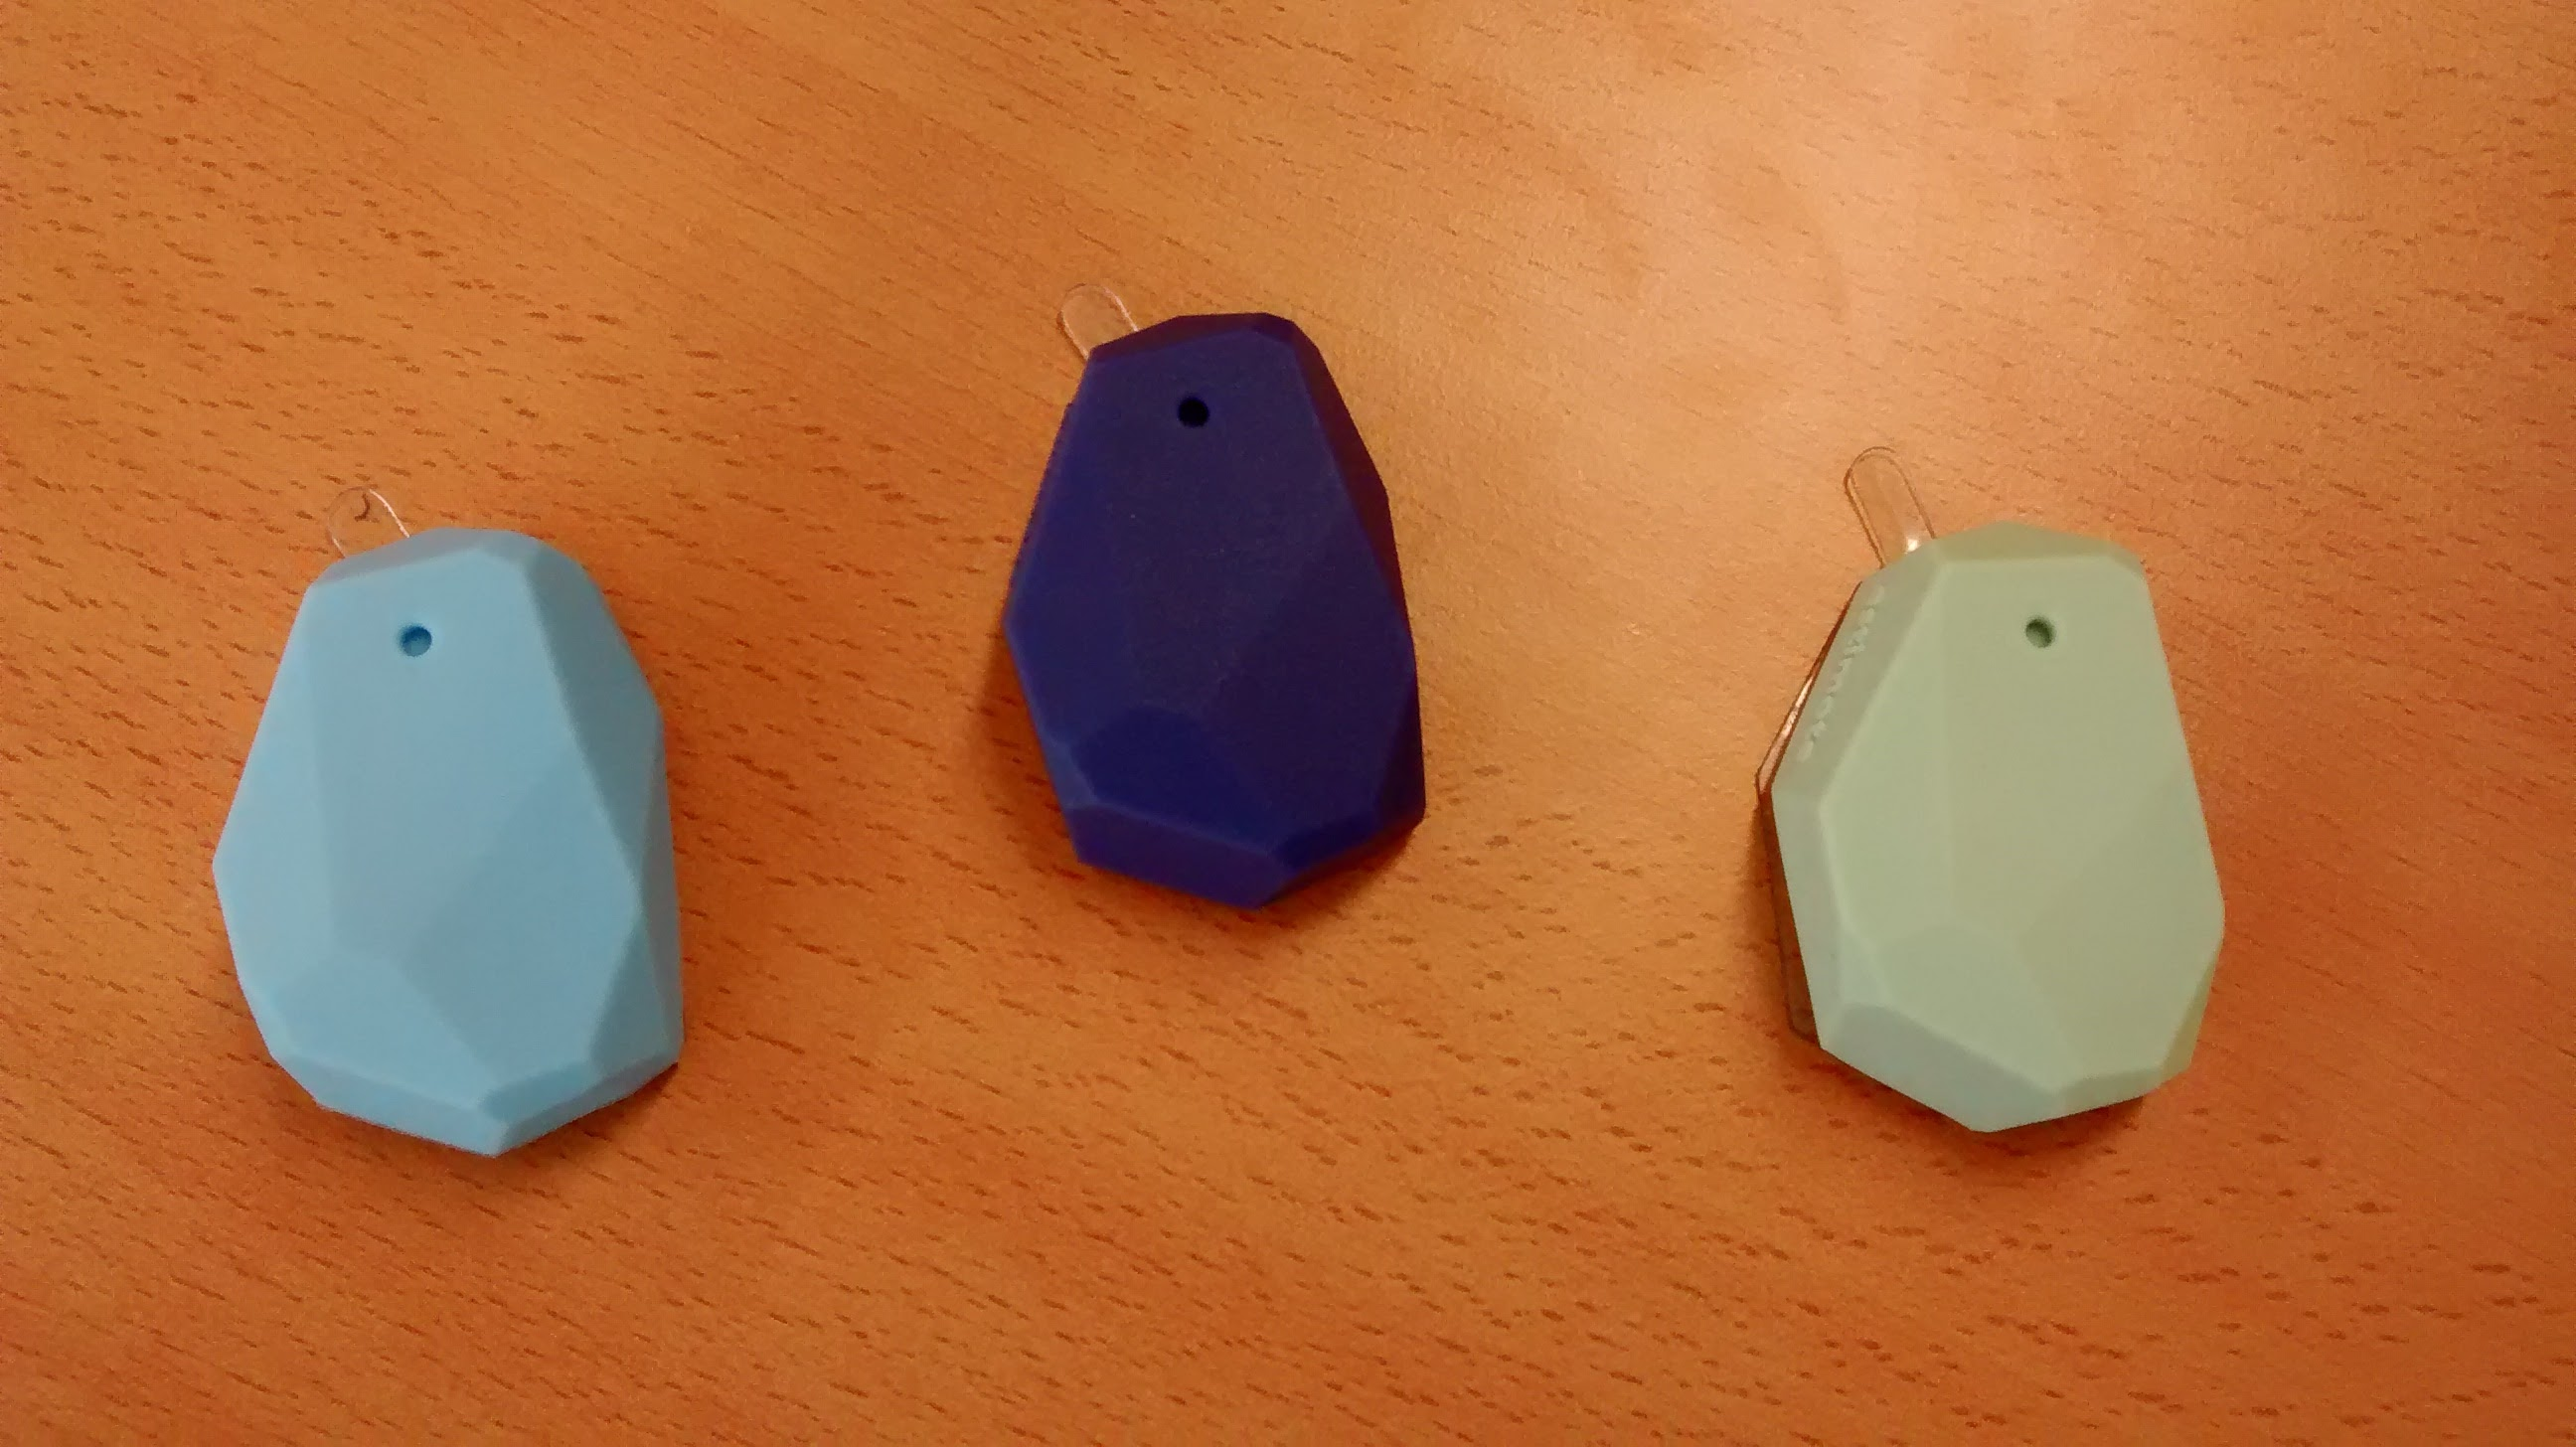
\includegraphics[width=0.5\textwidth, keepaspectratio]{images/estimote}
    \caption[Estimote beacons]{Beacons from Estimote, that were used during the implementation}
    \label{fig:estimote}
\end{figure}

\section{Backend}
\label{sec:implementation_backend}
% BaaS, Parse.com
% What it is
% How it works
% Collections created (UML?)
% SDKs used
As already mentioned, there was no implementation of the backend itself.
Using Parse \gls{BaaS}, in order to support the needs of this project, the following classes were
created, according to the data model in figure \ref{fig:backend_data_model}:
\begin{description}
  \item[Beacon]: Stores the information according to ibeacon protocol,
  which is \gls{UUID}, major and minor values. It also has a pointer
  to an instance of class User, which is a class provided by Parse \gls{BaaS} and represents its users. Fields such as, username, password, name and email are already provided by this class.
  Due to the existence of this class, the authentication mechanisms, such as, using username and password or using accounts from social networks, such as Facebook or Twitter, are already provided;
  A pointer to an instance of class User represents the user that owns the beacon;
  \item[Smart Place]: Stores information all smart places available,
  such as, name and description. It has a pointer to an instance of
  User, which is the user that created it;
  \item[Smart Place Instance]: When an owner wants to install a given
  Smart Place, he creates an instance of a Smart Place. Owners can
  customize the title and the message that appears in the users'
  mobile devices notifications;
  \item[Tag]: A Tag has a \gls{JSON} object and has pointers to instances
  of Smart Place Instance and Beacon classes. With this pointers, when
  the end users app detects a beacon, it is possible to send a query to
  the backend in order to get the tag that is associated to that beacon.
\end{description}

\begin{figure}[!ht]
  \centering
    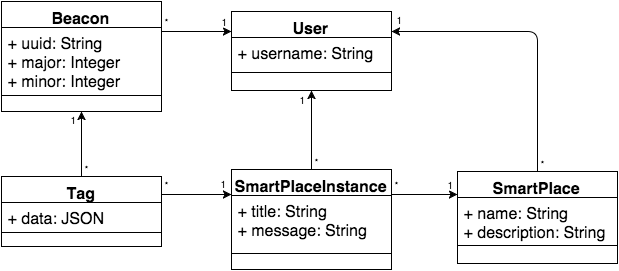
\includegraphics[width=0.5\textwidth]{images/backend_data_model}
    \caption[Data model]{Data model stored in Parse \gls{BaaS}}
    \label{fig:backend_data_model}
\end{figure}

Parse \gls{BaaS} has \glspl{SDK} available to many platforms and programming
languages, such as, Android, iOS, Javascript, etc.
In order to be able to make requests to the backend from the mobile apps and
from the Javascript API
the Parse Android and Javascript \glspl{SDK} were used.

\section{Smart Places}
\label{sec:implementation_smart_places}
% What are Smart Places
% Where they Run
A Smart Place has tags that provide a proximity-based service.
The Smart Restaurant and Smart Museum, presented in chapter \ref{chapter:solution}, section \ref{sec:solution_examples}, are examples of Smart Places.
They were developed according to our definition of Smart Place.
As also presented in chapter \ref{chapter:solution}, there is a mobile app that allows users to have access to these proximity-based services.
However, these services could be mobile apps themselves.
We could create an \gls{SDK}, for each platform, to allow developers to introduce proximity-based developers in their apps.
Following this approach, we would have a situation where the users would need to install one app for each Smart Place they want to use.
In order to understand why we have an app to access any Smart Place, we need first, to compare the possible approaches.

% How can be done (native or web)
% Compare both approaches
% Choose web
% Why
We could allow Smart Places to be native mobile apps or web apps that run inside an embedded web browser.
A native mobile app is an app, developed with the native tools, already provided by the platform.
This kind of apps only run in the platform that they were created for.
A web app is an application that runs inside a web browser. It can run in any platform that has a web browser available.
Table~\ref{tab:native_vs_web} compares native and web apps, showing the advantages and limitations of each category of apps.
If Smart Places were developed as native apps, users would need to install one app for each one.
This approach would not allow them to discover new proximity-based services while they were walking.
To circumvent this limitation, we decided that Smart Places would exist as web applications.
This way, any web application can react to the existence of tags in a Smart Place. Also, it leads to a situation where the users only need one app to have access to any Smart Place, because, each one, is a web application that will run inside an embedded web browser in the users mobile app.

\begin{table}[h]
\centering
\begin{tabular}{|c|c|c|l}
\cline{1-3}
 & Native & Web &  \\ \cline{1-3}
\begin{tabular}[c]{@{}c@{}}Access to device's features \\ (Camera, accelerometer,etc)\end{tabular} & All & Limited &  \\ \cline{1-3}
Installation needs & \begin{tabular}[c]{@{}c@{}}Need to install\\ the app\end{tabular} & \begin{tabular}[c]{@{}c@{}}Only a web browser\\ is needed\end{tabular} &  \\ \cline{1-3}
\begin{tabular}[c]{@{}c@{}}Method for finding\\ the app\end{tabular} & App stores & URL &  \\ \hline
Updates & \begin{tabular}[c]{@{}c@{}}Users can choose\\ to not update the\\ app\end{tabular} & \begin{tabular}[c]{@{}c@{}}All users have\\ access to the same\\ version\end{tabular} &  \\ \cline{1-3}
Where it can run & \begin{tabular}[c]{@{}c@{}}Only on the platform\\ for which it was\\ developed for\end{tabular} & On any platform &  \\ \cline{1-3}
\end{tabular}
\caption[Native vs Web apps]{A comparison of some characteristics of Native and Web mobile apps}
\label{tab:native_vs_web}
\end{table}


% WebView...
Having Smart Places as web applications accessed by the users mobile app, introduced in chapter \ref{chapter:solution}, section \ref{sec:solution_mobile_app_for_end_users}, is achieved by using the WebView\footnote{http://developer.android.com/guide/webapps/webview.html}, which is a widget, provided by the Android \gls{SDK} that allows to have web pages embedded inside any \gls{UI} in an Android application.
Smart Places are web applications that run in a WebView in the users mobile app.

% Data from native app to smart place running inside web view
Since we chose web apps as the mean to support Smart Places, somehow, they need to be able to detect nearby tags.
As it is possible to see, from Table~\ref{tab:native_vs_web}, web apps have limited access to the device's resources.
As described in section \ref{sec:implementation_tags}, \gls{BLE} beacons were used to support the existence of these tags.
How can a web application, running in an embedded web browser inside a native mobile app, detect tags in a Smart Place?
Our approach is to handle the tags, that is, the \gls{BLE} beacons and to pass the relevant information to the web application running inside the embedded web browser.
To do that, the native app invokes Javascript functions that exist in the embedded web browser, according to the \gls{API}, described in chapter \ref{chapter:solution}, section \ref{sec:solution_developers_api}.
To invoke Javascript code from the native app, a special \gls{URL} is loaded to the WebView.
The \gls{URL} is in the format: ``javascript:functionToInvoke(arguments)'', where ``functionToInvoke'' is the function we want to invoke inside the WebView and ``arguments'' is a list of arguments to pass to that function.

\section{Mobile applications}
\label{sec:implementation_mobile_applications}
% Mobile apps: Tools used, programming languages,
% -> Some kind of UML for each one
As already mentioned in section \ref{sec:implementation_tools}, we have used Android Studio to develop the mobile apps.
This development environment allows developers to create multiple
apps and modules inside the same project.
Taking this into account,
one project was created, with 2 apps and one library, as shown in figure
\ref{fig:smartplaces_package}. Since both apps use the Bluetooth receiver
of the mobile device and make requests to the backend, there is a library,
that both apps depend on, that offers some abstractions around the ibeacon
protocol and the communication with Parse.
Its implementation is detailed in section \ref{sub:implementation_library}

\begin{figure}[!ht]
  \centering
    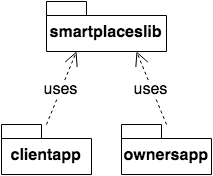
\includegraphics[width=0.5\textwidth, height=0.15\textheight,
      keepaspectratio]{images/smartplaces_package}
    \caption[Android project's structure]{Android project's structure}
    \label{fig:smartplaces_package}
\end{figure}

\subsection{Library}
\label{sub:implementation_library}
% Explain what the lib does
% UML for the lib
% Examples of its usage
As already mentioned, a library, smartplaceslib, as shown in figure \ref{fig:smartplaces_package}, was created in order to provide \glspl{API} that mobile apps can
use. Because, both apps use the Bluetooth receiver and interact with the backend, this library avoids having similar code in both apps. There are two important classes that this library offers:
\begin{description}
  \item[IBeaconsManager]: Offers methods to start scanning for beacons and change some settings such as, interval between each scan;
  \item[AbstractParseDataStore]: This class offers an abstraction of the Parse Android \gls{SDK}. It is extended by two classes, ClientParseDataStore, used in the end users mobile app, and OwnerParseDataStore, used in the owners mobile app. There are two different classes for each app because each app has different needs when interacting with the backend. Their common needs were encapsulated in methods in the AbstractParseDataStore class.
\end{description}

When IBeaconsManager class is used, it needs a BeaconScanCallback object, which overrides a method that is executed when beacons are scanned, because the scanning is an asynchronous process.
For instance, the code snippet in Listing~\ref{code:java_scan_beacons} illustrates how to use IBeaconsManager class, in a given
Activity\footnote{http://developer.android.com/guide/components/activities.html}, to scan for nearby beacons.

\begin{listing}[H]
  \begin{minted}[xleftmargin=.1\textwidth]{java}
  IBeaconsManager manager = new IBeaconsManager(this);
  manager.startScan(this, new BeaconScanCallback() {
    @Override
    public void beaconsFound(Collection<BeaconInfo> beacons) {
      // Code to be executed after beacons are found
    }
  })
  \end{minted}
  \caption[Java code for beacon scanning]{Java code in an Android Activity to scan for nearby beacons}
  \label{code:java_scan_beacons}
\end{listing}

\subsection{Mobile app for owners}
\label{sub:implementation_mobile_app_for_owners}
% Who are the owners
% Brief description of its features
% How it uses the library
% Android Studio, part of the project
As stated in chapter \ref{chapter:solution}, owners are the people who install beacons and configure Smart Places. This mobile Android app allows them to create an instance of a Smart Place.
In terms of backend, they are creating an instance of Smart Place Instance class, explained in \ref{sec:implementation_backend}.
In the android project it is called ownersapp and it uses the library, smartplaceslib, as shown in Figure \ref{fig:smartplaces_package}.
From the library, it uses the class IBeaconsManager to scan for nearby beacons and OwnersParseDataStore to allow owners to create Smart Place Instances and configure them.
The user interface tries to follow the conventions of Material Design\footnote{https://www.google.com/design/spec/material-design/introduction.html}, which is a design language, developed by \tm{Google}.
This language states some conventions about how to design an \gls{UI}.
Each \gls{UI} is implemented by a class that extends the Activity class, provided by the Android \gls{API}.
An Activity represents a single task, that the user can do, in an Android app.

\subsection{Mobile app for end users}
\label{sub:implementation_mobile_app_for_end_users}
% Who are the end users
% Brief description of its features
% How it uses the library
% Android Studio, part of the project
End users are the ones who actually use the Smart Places, that is, the users that have, in their mobile devices, an app that scans for nearby beacons and offer services provided by the Smart Places that were found.
It is part of the project, as clientapp, as shown in figure \ref{fig:smartplaces_package}. Simillary to the owners app, described in \ref{sub:implementation_mobile_app_for_owners}, it uses the smartplaceslib, to scan for nearby beacons and map them to the corresponding Smart Place Instances.
When Smart Place Instances are found, the app shows a notification for each one.
When the user click on the notification, the app calls an Activity that contains a WebView. This activity calls javascript functions on the WebView.
To ease that process, there is a class, SmartPlacesWebView that extends the original WebView class from the Android \gls{API}.
In that Activity, there is an instance of the IBeaconsManager class that will scan for nearby beacons in order to try to find tags. As mentioned in section \ref{sec:implementation_backend},
each instance of Tag has a \gls{JSON} object. That object must be sent to a Javascript function, for which, developers have defined a callback that will handle it. The SmartPlacesWebView has methods to invoke javascript code running inside the webview.
This way, the smart places app effectively combines the advantages of native apps with web apps, as compared in Section \ref{sec:implementation_smart_places}.

\section{Developers API}
\label{sec:implementation_developers_api}
% JS API
% Tools used (grunt, what is it and tasks used)
% Deployment process (using grunt)
% Make it available as a bower component
In this solution, developers create their Smart Places using web technologies, such as \gls{HTML}, \gls{CSS} and javascript, because they run inside a WebView in the clientapp, as mentioned in section \ref{sub:implementation_mobile_app_for_end_users}.
This is separated from the Android project, because it does not have any dependency from it.

This \gls{API} offer a global object, which is SmartPlaces, with several methods that developers use to define callbacks for some events. For instance, to define what happens when a tag is found, developers need to write code as shown in Listing~\ref{code:js_tag_found}:

\begin{listing}[H]
  \begin{minted}[xleftmargin=.1\textwidth]{javascript}
    SmartPlaces.onTagFound(function(tag) {
      // Code to handle when the mobile app detects a tag
    });
  \end{minted}
  \caption[Tag found]{Javascript code to define a callback when a tag is found}
  \label{code:js_tag_found}
\end{listing}

This library was developed in a modular way, that is, there are multiple javascript files, that, in the end, in the build process, are compiled in just one file.
To manage this build process, we used Grunt. There is a task that compiles all javascript files in just one, performs minification of that file and creates a new version, that is, creates a new tag in the repository and pushes those changes to it.

\section{Examples}
\label{sec:implementation_examples}
In order to make sure that the Javascript \gls{API} works as expected and that it can be applied to multiple kinds of smart places, two examples were implemented.
These examples try to be a proof of concept, that is, demonstrate that, using the Javascript API, a web application can be aware of nearby tags, in the real world, and execute useful computation using those tags.

\subsection{Smart Restaurant}
\label{sub:implementation_smart_restaurant}
% - what it is;
% - tools;
% - programming languages;
% - deployment;
% - overview of its structure
The idea of this Smart Place is to offer an easy way for customers, in a restaurant, to place their orders using their mobile devices.
We have used an existing solution created in the scope of a Master Thesis \cite{SLOC}.
It has a \gls{REST} \gls{API} written in \gls{PHP} language.
Our work here, was to create a frontend, that uses the Smart Places Javascript \gls{API} and the provided \gls{API}.
This frontend was written in \gls{HTML} and Javascript.
It was deployed in the web server of \gls{IST}. Simillary to Smart Places Javascript \gls{API}, the build process is managed by Grunt and there is a task to deploy this web application in the mentioned web server.

\subsection{Smart Museum}
\label{sub:implementation_smart_museum}
% - what it is;
% - tools;
% - programming languages;
% - deployment;
% - overview of its structure
The Smart Museum is another example that was created to use the Javascript \gls{API} and verify that we can apply it to multiple applications.
The main goal was to show some information about some objects in a museum.

To work with real data instead of creating our own museum we have used a real data source.
The Walters Art Museum provides a \gls{REST} \gls{API} that any developer can use to get data about collections and objects.
To use this \gls{API}, we created an account, in the \gls{API}'s website\footnote{http://api.thewalters.org} and requested to get a token. This token is used in any request to allow the \gls{REST} \gls{API} to identify each individual request.

This web application was created using NodeJS\footnote{http://nodejs.org} with Express\footnote{http://expressjs.com} framework, that allow to create an \gls{HTTP} server using javascript.
It is currently deployed on Heroku\footnote{http://www.heroku.com} which is a cloud \gls{PaaS}, that supports many programming languages and development stacks.
Simillary to the other example, in section \ref{sub:implementation_smart_restaurant}, this one also uses Grunt to manage the build process. Before the deployment, all javascript files that will run on the browser are concatenated in one file. Then, that file is minified.

\section{Summary}
\label{sec:implementation_summary}
% Explained implementation of solution componens presented in previous chapter
In the previous chapter, we introduced our solution and the main components that are part of it.
Here, we looked at each component and described its implementation.

% Tools
% -> Java tools (Android Studio)
% -> JS tools (Grunt, bower)
First, there is a summary of the tools used in the development of this solution.
Android Studio was used to develop the two mobile apps, for owners and end users.
For the developers \gls{API} and the Smart Restaurant and Smart Museum examples, Grunt and Bower were used.
Grunt is a tool to manage the build process of frontend assets, such as, Javascript files.
There are many tasks to handle Javascript files concatenation and minification.
Bower is a dependency management tool for frontend dependencies, that allows developers to specify the dependencies of their web applications instead of downloading each one manually.

% Tags
% -> Chose BLE beacons
% -> why
Another important component of our solution are the tags that are deployed in a given Smart Place.
We decided to use \gls{BLE} beacons using ibeacon protocol, because nowadays, most of the smartphones are \gls{BLE} enabled.
Our solution does not require the user to acquire any extra hardware, besides his mobile device.

% Backend
% -> Used Parse BaaS
% -> Brief domain model
Our solution stores information in a backend.
Instead of developing this component from the scratch, we have used a \gls{BaaS}, which allowed us to only be concerned about the data model and not with the typical concerns of a distributed system, such as, scalability, performance and deployment.
In our data model, there is the concept of Smart Place. When owners configure a given Smart Place, they are creating a Smart Place Instance.
Smart Place Instances have tags, which are represented by beacons.

% Smart Places
% -> Native vs Web
% -> Why web
Smart Places provide proximity-based services, that could be supported through native or web apps.
Native apps are installed on the mobile device's \gls{OS} and only run on the \gls{OS} they are developed for.
Web apps run on any platform where a web browser can run.
We discussed the advantages and limitations of native and web apps.
The final decision was to have an embedded web browser, inside the mobile app for end users, that would allow to have access to any Smart Place without requiring users to install a native app for each one.
The mobile app scans for nearby beacons and send the needed data to the Smart Place, running inside the embedded web browser.

% Mobile applications
% -> library (what and why)
% -> Mobile app for owners (used library, Android Studio)
% -> Mobile app for end users (used library, Android Studio)
We have used Android Studio to develop the two mobile apps.
However, both apps needed to scan for nearby beacons and make requests to the backend.
Inside the same project, we create a library, from which the two apps depend, in order to avoid having repeated code in both apps.

% Developers API
% -> JS library
% -> Why JS
Since Smart Places are web apps, we have developed a Javascript library.
This library offers an \gls{API} to handle the events sent by the mobile apps, for instance, when a tag is found.
Due to the fact that the mobile apps send events to the Smart Place running in the embedded web browser, this \gls{API} is asynchronous and its methods require callback functions as arguments.

% Examples
% -> Introduced in previous chapters
% -> Developed using web technologies
The Smart Restaurant and Smart Museum were implemented using web technologies, such as, \gls{HTML}, \gls{CSS} and Javascript.
These examples contributed to the development of Developers \gls{API}.
While developing the Smart Restaurant, we wrote Javascript code to handle the events sent by the native mobile apps.
From this code, it was possible to define an \gls{API} that was released as a separated library.
This library was used successfully in the Smart Museum example.
